%\FloatBarrier
\section{Experimental Evaluation}
\label{sec:experiments}

\subsection{Experimental Setup}
\label{sec:setup}





\begin{figure*}[!t]
    \centering
    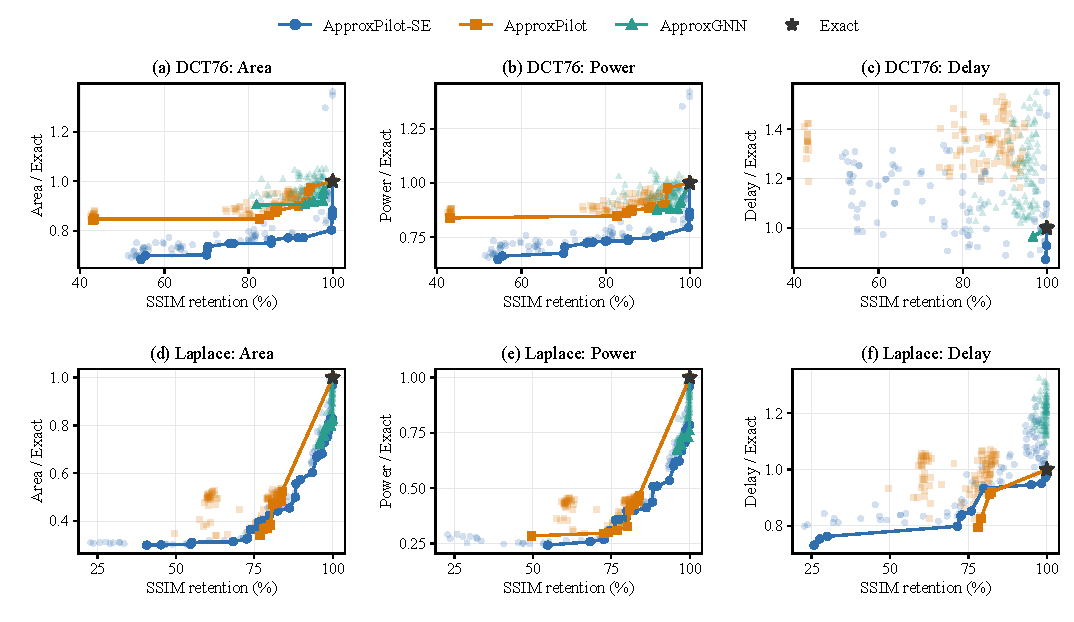
\includegraphics[width=\textwidth]{figures/measured_pareto.pdf}
    \caption{Measured PPA--QoR tradeoffs on DCT76 and Laplace.
    All plotted points correspond to final candidate designs evaluated
    using logic synthesis and application-level QoR evaluation.
    Faint markers show measured candidates, and connected markers show
    the two-dimensional nondominated fronts. Stars indicate the Exact designs.}
    \label{fig:measured_pareto}
\end{figure*}




Five approximate-accelerator benchmarks are considered: DCT, Laplace, Sobel, Gaussian, and KMeans, covering different arithmetic compositions and design-space sizes. For each benchmark, the legal Exact/Approximate configuration space is constructed according to the arithmetic operations and RTL interfaces of the target design. Table~\ref{tab:benchmarks} summarizes the benchmark characteristics.

\begin{table}[t]
\centering
\caption{Summary of the evaluated approximate-accelerator benchmarks.}
\label{tab:benchmarks}
\footnotesize
\setlength{\tabcolsep}{5pt}
\begin{tabular}{lcc}
\toprule
Benchmark & Arithmetic Operations & Configurable Sites \\
\midrule
DCT      & Add / Sub               & 76 \\
Laplace  & Add                     & 60 \\
Sobel    & Add / Sub               & 5  \\
Gaussian & Add / Mul               & 17 \\
KMeans   & Add / Sub / Mul / Sqrt  & 16 \\
\bottomrule
\end{tabular}
\end{table}

Candidate designs are synthesized using Synopsys Design Compiler with the FreePDK45 45-nm standard-cell library, from which system-level Area, Power, and Delay are obtained. Application quality is evaluated on BSDS500 images~\cite{arbelaez2011contour} using the structural similarity index (SSIM)~\cite{wang2004ssim}. DCT76 uses eight grayscale images, with SSIM measured between the reconstructed output and the input image. SSIM retention is the ratio of a candidate's mean SSIM to that of the corresponding Exact design. Final PPA and QoR results are obtained from logic synthesis and application execution.

ApproxPilot-SE is compared with ApproxPilot and ApproxGNN. Each method retains its own surrogate and search strategy over the same legal configuration space and system-level evaluation flow. On DCT76, each method uses 900 training configurations, a common 60-configuration validation set, and 15,000 final search trials with seed 101. Each final archive contains 100 measured candidates and Exact; training and validation configurations are excluded. ApproxPilot retains its critical-path supervision, and ApproxGNN uses its official pretrained component embeddings. DCT76 is also used to analyze co-evolving DSE, surrogate ranking quality, and Delay modeling.

Area, Power, and Delay are normalized to the Exact design of each benchmark. PPA tradeoffs are evaluated under SSIM-retention constraints of 80\%, 85\%, 90\%, 95\%, and 99\%, and three-dimensional hypervolume (HV) is used to quantify the Pareto region satisfying each quality constraint. The additional tradeoff space beyond the Exact design is reported as HV Gain:

\begin{equation}
    \mathrm{HV}_{\mathrm{gain}}
    =
    \mathrm{HV}
    \left(
        \mathcal{S}\cup\{\mathrm{Exact}\};\mathbf{r}
    \right)
    -
    \mathrm{HV}
    \left(
        \{\mathrm{Exact}\};\mathbf{r}
    \right),
    \label{eq:hv_gain}
\end{equation}

where $\mathcal{S}$ denotes the set of measured candidates satisfying the corresponding SSIM-retention constraint, and $\mathbf{r}=(1.10,1.10,1.70)$ is the reference point in the normalized PPA space. The same normalization and metric definitions are applied to all methods within each benchmark.
























\subsection{Design Space Exploration}
\label{sec:dse_results}

We evaluate the end-to-end optimization quality of
ApproxPilot-SE against ApproxPilot and ApproxGNN using
measured PPA--QoR tradeoffs and quality-constrained HV Gain.



Fig.~\ref{fig:measured_pareto} presents the measured PPA--QoR
tradeoffs on DCT76 and Laplace. Each point corresponds to a
final candidate evaluated using the complete ground-truth flow.
The projected fronts provide a direct view of how the three
methods distribute verified designs across different hardware-cost
and output-quality regions.

On DCT76, ApproxPilot-SE maintains verified PPA improvements
over a broad range of SSIM retention. Its candidates extend the
measured tradeoff region not only at relatively relaxed quality
constraints, but also near the Exact-quality region. This is
important because the feasible region becomes progressively
narrower as the SSIM-retention requirement increases, leaving
fewer configurations that can simultaneously improve Area,
Power, and Delay.

On Laplace, ApproxPilot-SE provides a broad range of measured
tradeoffs, with its strongest HV gains relative to the baselines
at the 85\%--95\% retention constraints.

To quantify these tradeoffs across all evaluated benchmarks,
we use the verified 3-D PPA hypervolume gain over the Exact
design. Area, Power, and Delay are normalized to the
corresponding Exact implementation, while SSIM retention is
used as a feasibility constraint. The reported metric measures
the additional 3-D PPA hypervolume contributed by verified
approximate designs beyond the Exact reference.

\begin{table*}[!t]
\centering
\caption{Verified 3-D PPA hypervolume gain over the Exact design
under different SSIM-retention constraints.}
\label{tab:verified_hv_all}
\footnotesize
\renewcommand{\arraystretch}{1.08}

\begin{tabular*}{\textwidth}
{@{\extracolsep{\fill}} l l c c c c c @{}}
\toprule
\textbf{Benchmark} &
\textbf{Method} &
\textbf{80\%} &
\textbf{85\%} &
\textbf{90\%} &
\textbf{95\%} &
\textbf{99\%} \\
\midrule

\multirow{3}{*}{DCT}
& ApproxPilot
& 0.027075
& 0.021521
& 0.016160
& 0.000000
& 0.000000 \\
& ApproxGNN
& 0.024394
& 0.023273
& 0.023273
& 0.021611
& 0.000000 \\
& \textbf{ApproxPilot-SE}
& \textbf{0.095285}
& \textbf{0.092657}
& \textbf{0.085054}
& \textbf{0.067996}
& \textbf{0.067996} \\

\midrule

\multirow{3}{*}{Laplace}
& ApproxPilot
& \textbf{0.422106}
& 0.000000
& 0.000000
& 0.000000
& 0.000000 \\
& ApproxGNN
& 0.088416
& 0.088416
& 0.088416
& 0.088416
& \textbf{0.061240} \\
& \textbf{ApproxPilot-SE}
& 0.338411
& \textbf{0.325134}
& \textbf{0.188793}
& \textbf{0.138231}
& 0.053628 \\

\midrule

\multirow{3}{*}{Gaussian}
& ApproxPilot
& 0.290535
& 0.236497
& 0.186049
& 0.082716
& 0.000000 \\
& ApproxGNN
& \textbf{0.295673}
& 0.120928
& 0.055735
& 0.020681
& 0.004514 \\
& \textbf{ApproxPilot-SE}
& 0.258298
& \textbf{0.258298}
& \textbf{0.258298}
& \textbf{0.083437}
& \textbf{0.081900} \\

\midrule

\multirow{3}{*}{Sobel}
& ApproxPilot
& 0.208729
& 0.133068
& 0.081493
& 0.069325
& 0.008950 \\
& ApproxGNN
& \textbf{0.229965}
& 0.115541
& 0.054248
& 0.054248
& 0.009402 \\
& \textbf{ApproxPilot-SE}
& 0.208278
& \textbf{0.143541}
& \textbf{0.114777}
& \textbf{0.085003}
& \textbf{0.016307} \\

\midrule

\multirow{3}{*}{KMeans}
& ApproxPilot
& 0.377168
& 0.019913
& 0.013244
& 0.005123
& \textbf{0.000746} \\
& ApproxGNN
& 0.479862
& 0.066604
& 0.013502
& 0.013500
& 0.000000 \\
& \textbf{ApproxPilot-SE}
& \textbf{1.571801}
& \textbf{0.315895}
& \textbf{0.248737}
& \textbf{0.124565}
& 0.000000 \\


\bottomrule
\end{tabular*}
\end{table*}

Table~\ref{tab:verified_hv_all} confirms the DCT76 trend
quantitatively. ApproxPilot-SE achieves the highest verified
HV Gain at every evaluated SSIM-retention level. At 90\%
retention, its HV Gain reaches 0.085054, compared with
0.023273 for the stronger baseline at the same constraint.
At 95\% and 99\% retention, ApproxPilot-SE retains an
HV Gain of 0.067996, whereas the baselines provide either
substantially smaller gains or no additional hypervolume beyond
the Exact reference.

On Laplace, ApproxPilot-SE gives the largest HV Gain at
85\%, 90\%, and 95\% retention, reaching 0.325134,
0.188793, and 0.138231, respectively. These operating points
offer designers substantial PPA tradeoffs while preserving
application quality.

On Gaussian, ApproxPilot-SE gives the largest HV Gain from
85\% through 99\% retention. At 90\% retention, it reaches
0.258298, compared with 0.186049 for ApproxPilot and
0.055735 for ApproxGNN. The difference remains visible at
99\% retention, where ApproxPilot-SE retains an HV Gain of
0.081900 while the two baselines reach 0 and 0.004514.

On Sobel, ApproxPilot-SE achieves the largest HV Gain from
85\% through 99\% retention. At 90\% retention, the gain increases
from 0.081493 for ApproxPilot and 0.054248 for ApproxGNN
to 0.114777 for ApproxPilot-SE. Under the 99\% constraint,
ApproxPilot-SE retains a gain of 0.016307, compared with
0.008950 and 0.009402 for ApproxPilot and ApproxGNN,
respectively.

Across these benchmarks, the most notable pattern appears in
the higher-quality region. ApproxPilot-SE more frequently
preserves useful verified Pareto volume as the SSIM-retention
constraint becomes stricter. This is the region in which the
search must distinguish among configurations whose application
quality is already close to Exact while still identifying
meaningful hardware improvements.

The final archive also provides individual designs with simultaneous
PPA savings at high output quality. Table~\ref{tab:dct_case} presents
one such DCT76 configuration.

\begin{table}[!t]
\centering
\caption{Representative high-quality ApproxPilot-SE design on DCT76.}
\label{tab:dct_case}
\footnotesize
\setlength{\tabcolsep}{4.2pt}
\renewcommand{\arraystretch}{1.08}
\begin{tabular*}{\columnwidth}{@{\extracolsep{\fill}} lccc @{}}
\toprule
\textbf{Metric} &
\textbf{Exact} &
\textbf{ApproxPilot-SE} &
\textbf{Reduction} \\
\midrule
Area ($\mu$m$^2$)
& 3498.166
& 2807.896
& 19.73\% \\
Power (mW)
& 1.421650
& 1.130239
& 20.50\% \\
Delay (ns)
& 2.797612
& 2.442155
& 12.71\% \\
Mean SSIM
& 0.855541
& 0.852843
& -- \\
SSIM Retention
& 100\%
& 99.68\%
& -- \\
\bottomrule
\end{tabular*}
\end{table}

As shown in Table~\ref{tab:dct_case}, the selected design
retains 99.68\% of the Exact-design SSIM while reducing
Area, Power, and Delay by 19.73\%, 20.50\%, and 12.71\%,
respectively. Among the 76 configurable arithmetic sites,
38 remain Exact and 38 use approximate implementations,
while the four structurally fixed Exact nodes remain unchanged.
This configuration combines savings in all three hardware objectives
with output quality close to Exact.

\begin{figure}[!t]
    \centering
    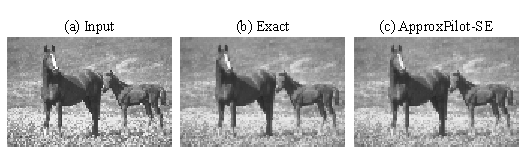
\includegraphics[width=\columnwidth]{figures/case_113016.pdf}
    \caption{Application outputs of the representative high-quality
    DCT76 design. ApproxPilot-SE retains 99.68\% of the
    mean Exact-design SSIM while simultaneously reducing Area, Power,
    and Delay.}
    \label{fig:dct_case}
\end{figure}

Fig.~\ref{fig:dct_case} provides a qualitative comparison of
the corresponding application outputs. The ApproxPilot-SE
output remains visually close to the Exact result while achieving
the PPA reductions reported in Table~\ref{tab:dct_case}.
Together with the verified hypervolume results, this example
shows that the final archive provides practical design choices
spanning both system-level hardware efficiency and
application-level quality.

The following experiments analyze the mechanisms that support
these end-to-end results. We first isolate the effect of
co-evolving surrogate updates during DSE, and then examine
surrogate ranking quality and the timing-domain Delay readout.













%Effect of Co-Evolving DSE
\subsection{Effect of Co-Evolving DSE}
\label{sec:coevolving}

The value of co-evolving DSE lies in where the ground-truth evaluation budget is allocated. We compare it with a One-shot variant using the same surrogate architecture, 900 training labels, and 60 validation configurations. One-shot trains on a method-independent sample of 900 configurations before DSE. ApproxPilot-SE starts from a 540/60 training--validation split (9:1) and acquires 90 configurations in each of four feedback rounds, each with 2,000 surrogate search trials. Both workflows then use 15,000 final search trials and verify 100 candidates plus Exact.

\begin{figure}[!t]
    \centering
    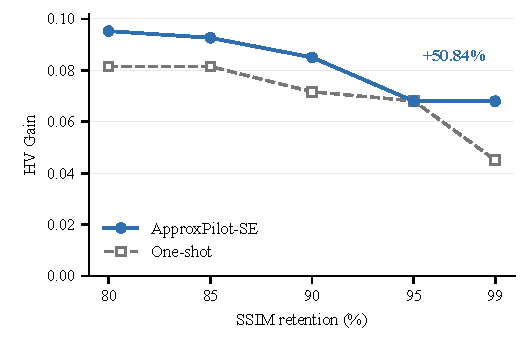
\includegraphics[width=\columnwidth]{figures/coevolving_hv_gain.pdf}
    \caption{Measured HV Gain of ApproxPilot-SE and the aligned One-shot variant under the same target-system training-label budget.}
    \label{fig:coevolving_hv}
\end{figure}

Fig.~\ref{fig:coevolving_hv} compares the measured HV Gain obtained under different SSIM-retention constraints. At 80\%, 85\%, and 90\% retention, ApproxPilot-SE improves HV Gain over One-shot by 16.91\%, 13.69\%, and 18.68\%, respectively. The separation becomes substantially larger under the strictest quality constraint. At 99\% retention, One-shot achieves an HV Gain of 0.045079, whereas ApproxPilot-SE reaches 0.067996, corresponding to a 50.84\% improvement.

Co-evolving DSE directs new system-level measurements toward the Pareto-relevant configurations exposed by search. Updating both surrogates with these measurements lets subsequent rounds refine the same regions, coupling the allocation of training labels to the optimization objective.

At 99\% SSIM retention, the feasible designs must preserve output quality close to Exact. ApproxPilot-SE retains an HV Gain of approximately 0.068 in this region, showing that search-guided label acquisition yields useful PPA tradeoffs under a stringent quality constraint.












%Surrogate Ranking under Limited Labels
%Surrogate Ranking Quality
\subsection{Surrogate Ranking Quality}
\label{sec:surrogate_ranking}

Pareto selection depends on rankings across Area, Power, Delay,
and SSIM. We compare their Spearman correlations at 180, 540,
and 900 training configurations using a common 60-configuration
validation set.

\begin{table}[t]
\centering
\caption{Spearman ranking correlation on the DCT76 validation set.}
\label{tab:surrogate_ranking}
\footnotesize
\setlength{\tabcolsep}{3pt}
\renewcommand{\arraystretch}{1.08}

\begin{tabular*}{\columnwidth}
{@{\extracolsep{\fill}} c l c c c c c @{}}
\toprule
\textbf{Labels} &
\textbf{Method} &
\textbf{A} &
\textbf{P} &
\textbf{D} &
\textbf{Q} &
\textbf{Min.} \\
\midrule

\multirow{3}{*}{180}
& ApproxPilot
& 0.898 & 0.813 & 0.860 & 0.831 & 0.813 \\
& ApproxGNN
& 0.069 & 0.119 & 0.712 & 0.757 & 0.069 \\
& ApproxPilot-SE
& \textbf{0.913}
& \textbf{0.884}
& \textbf{0.866}
& \textbf{0.926}
& \textbf{0.866} \\

\addlinespace[2pt]

\multirow{3}{*}{540}
& ApproxPilot
& 0.920 & 0.850 & 0.885 & 0.900 & 0.850 \\
& ApproxGNN
& 0.168 & 0.156 & 0.701 & 0.867 & 0.156 \\
& ApproxPilot-SE
& \textbf{0.938}
& \textbf{0.908}
& \textbf{0.888}
& \textbf{0.929}
& \textbf{0.888} \\

\addlinespace[2pt]

\multirow{3}{*}{900}
& ApproxPilot
& \textbf{0.963}
& 0.881 & 0.896 & 0.912 & 0.881 \\
& ApproxGNN
& 0.162 & 0.601 & 0.714 & 0.893 & 0.162 \\
& ApproxPilot-SE
& 0.956
& \textbf{0.941}
& \textbf{0.920}
& \textbf{0.949}
& \textbf{0.920} \\

\bottomrule
\end{tabular*}
\par\smallskip
\raggedright A/P/D/Q: Area/Power/Delay/SSIM; Min.: lowest correlation across the four objectives. Bold denotes the highest value at each training size.
\end{table}

With 180 target-system labels, ApproxPilot-SE achieves Spearman
correlations of 0.9126, 0.8835, 0.8664, and 0.9255 for Area,
Power, Delay, and SSIM, respectively, with a minimum correlation
of 0.8664 across all four objectives. At 540 labels,
the corresponding correlations increase to 0.9375, 0.9079,
0.8876, and 0.9290.

At 900 labels, ApproxPilot-SE reaches 0.9557, 0.9412, 0.9202,
and 0.9487 across the four objectives, with a minimum correlation
of 0.9202 and the highest correlations on Power, Delay, and SSIM.

ApproxPilot-SE provides balanced ranking quality across all four
DSE objectives. This property supports Pareto selection, which
compares configurations jointly by hardware cost and output quality.

\begin{figure*}[t]
    \centering
    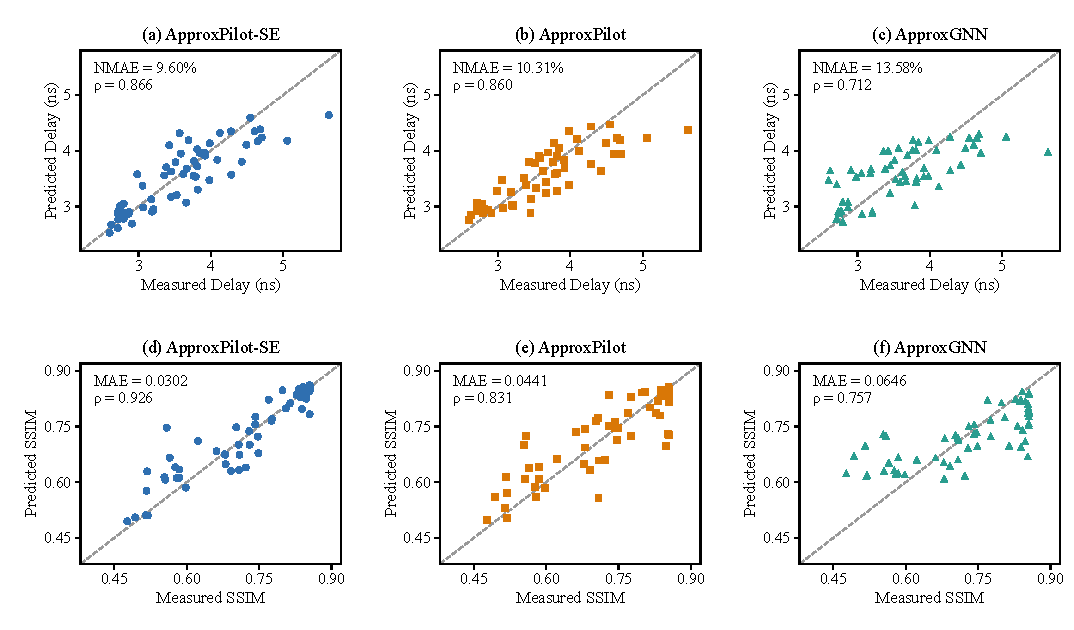
\includegraphics[width=\textwidth]{figures/pred_vs_truth_dct76.pdf}
    \caption{Prediction-versus-ground-truth comparison on DCT76
    with 180 training configurations and 60 validation configurations. The top row shows Delay
    prediction and the bottom row shows SSIM prediction for
    ApproxPilot-SE, ApproxPilot, and ApproxGNN.}
    \label{fig:pred_vs_truth}
\end{figure*}

Fig.~\ref{fig:pred_vs_truth} visualizes Delay and SSIM predictions
under the 180-label setting. Delay NMAE is MAE divided by Exact Delay.
For Delay, ApproxPilot-SE achieves an NMAE of 9.60\% and a
Spearman correlation of 0.866, compared with 10.31\% and 0.860
for ApproxPilot, and 13.58\% and 0.712 for ApproxGNN.
For SSIM, ApproxPilot-SE achieves an MAE of 0.0302 and a
Spearman correlation of 0.926, outperforming ApproxPilot
(0.0441, 0.831) and ApproxGNN (0.0646, 0.757).

The close agreement with measured Delay and SSIM in
Fig.~\ref{fig:pred_vs_truth}, together with the Area and Power
correlations in Table~\ref{tab:surrogate_ranking}, supports the
surrogate ensemble's ability to rank candidate designs with
180 target-system training labels.


















%Timing-Domain Delay Modeling
\subsection{Timing-Domain Delay Modeling}
\label{sec:delay_ablation}

The Delay objective differs from Area and Power because it is
strongly affected by the ordering and interaction of operations
along combinational paths. To evaluate whether the proposed
timing-domain path aggregation contributes useful structural
information beyond a conventional graph-level readout, we compare
it with a Global Max variant. The two models use the same graph
encoder, training data, optimization settings, and Delay targets;
the only difference is the readout used to construct the
configuration-level representation for Delay prediction.

The evaluation set is formed by the union of the final candidates
generated by ApproxPilot-SE, ApproxPilot, ApproxGNN, and the aligned
One-shot workflow. After removing the Exact design and duplicate
configurations, the set contains 400 configurations with measured
system-level Delay. Both variants use 900 training and 60 validation
configurations with paired seeds 101, 202, and 303. The mean and sample standard
deviation are reported in Table~\ref{tab:delay_ablation}.

\begin{table}[t]
\centering
\caption{Ablation of the Delay readout on DCT76. Mean $\pm$ sample standard deviation over three paired seeds.}
\label{tab:delay_ablation}
\footnotesize
\setlength{\tabcolsep}{4pt}
\renewcommand{\arraystretch}{1.08}

\begin{tabular*}{\columnwidth}{@{\extracolsep{\fill}} lcc @{}}
\toprule
\textbf{Metric}
& \textbf{Global Max}
& \textbf{Timing-Domain Path} \\
\midrule
MAE (ns)$\downarrow$
& $0.2095 \pm 0.0102$
& $\mathbf{0.1939 \pm 0.0022}$
\\
Spearman $\rho$$\uparrow$
& $0.7965 \pm 0.0206$
& $\mathbf{0.8217 \pm 0.0228}$
\\
Pairwise Acc. (\%)$\uparrow$
& $80.37 \pm 0.88$
& $\mathbf{81.67 \pm 1.19}$ \\
\bottomrule
\end{tabular*}

\end{table}

The timing-domain path readout improves all three Delay metrics.
Its MAE decreases from 0.2095~ns to 0.1939~ns, corresponding to
a 7.45\% reduction. At the same time, Spearman correlation
increases from 0.7965 to 0.8217, indicating a better ranking of
candidate configurations by measured Delay. Pairwise ranking
accuracy also improves from 80.37\% to 81.67\%.

These results are consistent with the role of the proposed readout
in Section~\ref{sec:method}. Global Max pooling treats node
representations as an unordered set and retains only the strongest
response in each feature dimension. In contrast, timing-domain
path aggregation propagates encoded node states along directed RTL
dependencies before the final aggregation. The resulting
representation therefore preserves information about upstream
operation sequences and competing paths, which is directly
relevant to configuration-level Delay.

The readout thus improves both Delay estimates and the ordering
of candidate designs used by multiobjective search.
